\chapter{\texorpdfstring{\ds/\dpl production-yield ratio}{Ds+/D+ production-yield ratio}}\label{ch:results}
The \pt-differential \ds/\dpl production-yield ratio can be evaluated using the raw yields and the correction factors obtained in Chapters~\ref{chap:RY} and~\ref{ch:corrections}. The \ds/\dpl production-yield ratio is defined using Eq.~\ref{eq:DsDplusRatio}, here reported for convenience:
\begin{equation*}
    \ds/\dpl = \frac{N_\mathrm{raw}^{\ds}\cdot \fpds}{\aeffpds \cdot \mathrm{BR}^\ds} \cdot \left(\frac{N_\mathrm{raw}^{\dpl}\cdot \fpdpl}{\aeffpdpl \cdot \mathrm{BR}^\dpl}\right)^{-1}\quad .
\end{equation*}
Previous measurements of this ratio have been performed in pp collisions at different centre-of-mass energies and rapidity windows, and it is therefore interesting to investigate whether the \ds/\dpl production-yield ratio depends on either of these variables. In addition, several models have been developed to describe the production of the two D-meson species in pp collisions. They are all based on perturbative QCD calculations for the description of the charm-quark production in the hard-scattering processes (although through different approaches), but differ in the description of the parton shower and hadronisation process, as discussed in Chapter~\ref{ch:openHF}. The prompt \ds/\dpl production-yield ratio is a sensitive probe of the hadronisation mechanism of charm quarks, and the comparison between the measured values and the predictions from these models can be used to test their validity. Furthermore, these results provide a baseline for analogous measurements in Pb--Pb collisions.

Using the factorisation theorem~\cite{Collins:1989gx}, from Eq.~\ref{eq:pp_xsec}, the \ds/\dpl production-yield ratio is sensitive to the fragmentation functions of the charm quark into the two D-meson species, as the description of the parton distribution functions of the colliding protons and the charm production in the partonic scattering is the same for the two D-meson species. The ratio of the \pt-differential cross-sections of the two D-meson species can be expressed as:
\begin{equation*}
    \frac{\left.\frac{\de^2\sigma}{\de\pt\de y}\right\vert^\ds_\mathrm{prompt}}{\left.\frac{\de^2\sigma}{\de\pt\de y}\right\vert^\dpl_\mathrm{prompt}} = \frac{\int \de z D_\mathrm{c\rightarrow \ds}(z,\mu_\mathrm{F}^2)}{\int \de z D_\mathrm{c\rightarrow \dpl}(z,\mu_\mathrm{F}^2)} = \frac{f_\mathrm{c\rightarrow\ds}}{f_\mathrm{c\rightarrow\dpl}}\quad ,
\end{equation*}
where $D_\mathrm{c\rightarrow \ds (\dpl)}(z,\mu_\mathrm{F}^2)$ are the fragmentation functions of the charm quark for the hadronisation into a \ds (\dpl) meson and their integrals with respect to $z$, $f_\mathrm{c\rightarrow\ds(\dpl)}$, are called \emph{fragmentation fractions}. These studies therefore provide information on the energy and rapidity dependence of the fragmentation functions, and, potentially, constraints for these quantities, which are crucial ingredients for the perturbative calculation of the open-charm hadron production cross-section in pp collisions in the framework of the factorisation theorem. 

The \pt-differential \ds/\dpl production-yield ratio measured in this Thesis at midrapidity \mbox{($\lvert y\rvert<0.5$)} in pp collisions at \thirteen with the ALICE detector is shown in Fig.~\ref{fig:dsdplratio}. The statistical uncertainties are reported using vertical bars, while the systematic uncertainties are shown as boxes. The results present a steeply-increasing \ds/\dpl production-yield ratio between the first two \pt intervals, followed by a flat trend with \pt for $\pt>1$~\gevc. 


\begin{figure}[tb]
    \centering
    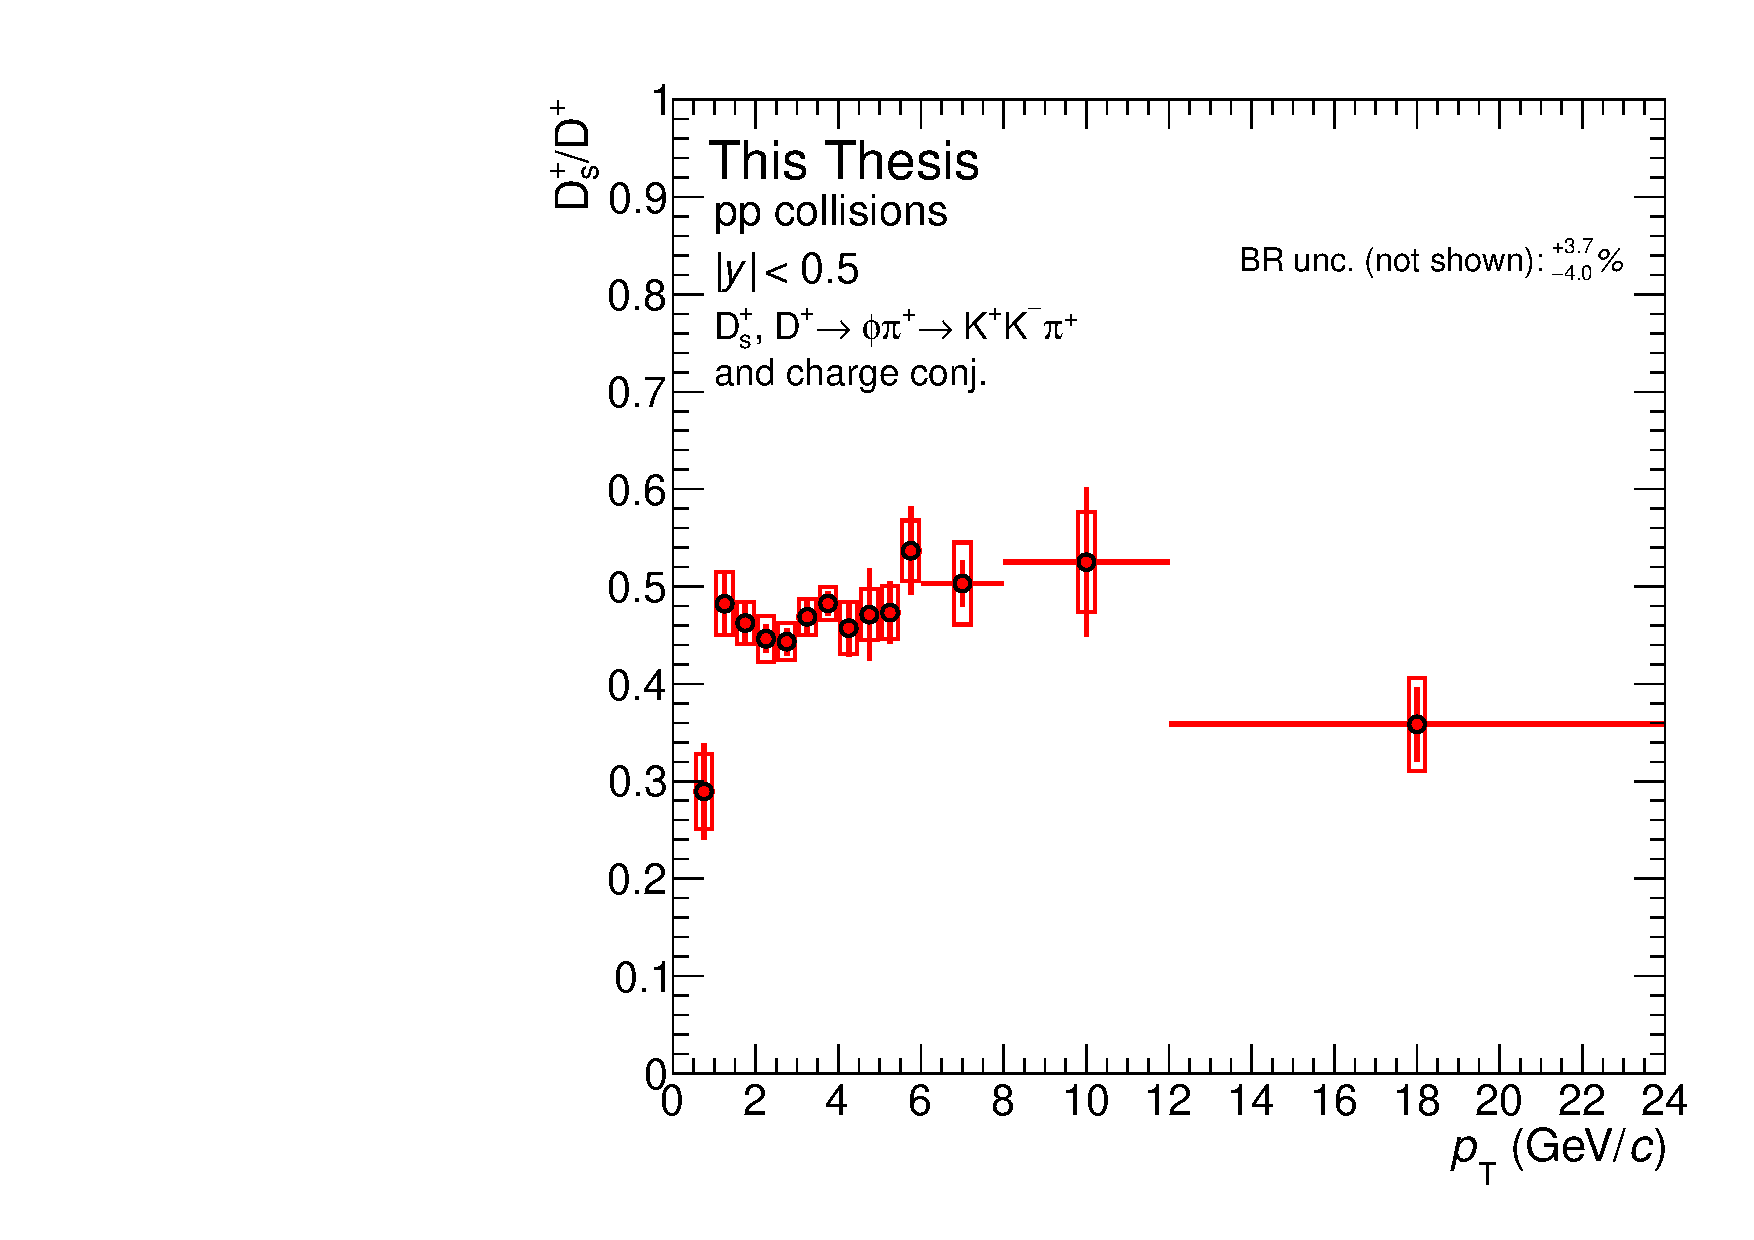
\includegraphics[width=0.7\textwidth]{Figures/Chapter 7/DsOverDplus.pdf}
    \caption{\pt-differential \ds/\dpl production-yield ratio measured in this Thesis at midrapidity ($\lvert y\rvert<0.5$) in pp collisions at \thirteen with the ALICE experimental apparatus.}
    \label{fig:dsdplratio}
\end{figure}

\section{Dependence on centre-of-mass energy}
Measurements performed in heavy-ion collisions at the SPS observed an enhancement in the production of strange hadrons with respect to non-strange hadrons~\cite{WA97:1999uwz,NA57:2010tnk}, which was attributed to the modification of the hadronisation process in the QGP and the augmented thermal production of strange quarks as compared to pp collisions owing to the high temperatures reached in the medium. At the LHC, measurements performed in pp, p--Pb, and Pb--Pb collisions by the ALICE Collaboration~\cite{ALICE:2016fzo,ALICE:2013xmt,ALICE:2015mpp} showed that the phenomenon of strangeness enhancement is also present in small collision systems, in high charged-particle multiplicity collisions. The $\mathrm{K^0_s/\pi}, \Lambda/\pi, \Xi/\pi$, and $\Omega/\pi$ production-yield ratios were observed to follow a smoothly increasing trend with multiplicity from pp to Pb--Pb collisions. This behaviour is described by different models (such as \textsc{Pythia} with colour-reconnection plus rope hadronisation~\cite{Bierlich:2014xba}, Statistical Hadronisation Model~\cite{Andronic:2017pug}, and the Catania coalescence model~\cite{Minissale:2020bif}), which implement different approaches to describe the hadronisation process, but all assume the establishment of a parton-rich environment in the collision.

\begin{figure}[tb]
    \centering
    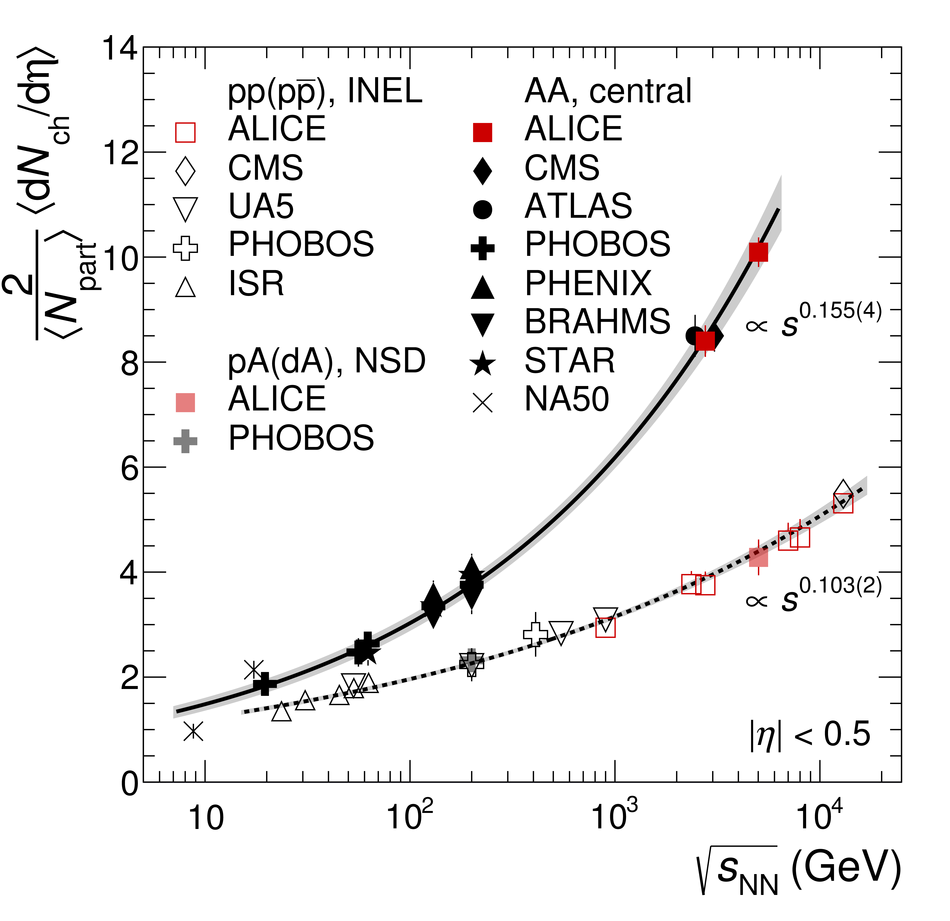
\includegraphics[width=0.7\textwidth]{Figures/Chapter 7/sqrtsFig-18534.png}
    \caption{Charged-particle multiplicity density, normalised to the number of nucleons participating in the collision divided by a factor 2 $\left(\langle N_\mathrm{part}\rangle/2\right)$ as a function of the centre-of-mass energy per nucleon pair of the collision for central nucleus-nucleus, proton-nucleus, and pp collisions. The $s_\mathrm{NN}$-dependence of the charged-particle multiplicity density is parametrised using a power-law function, and is shown with solid and dashed lines for cental nucleus-nucleus collisions and smaller collision systems, respectively. Figure taken from Ref.~\cite{ALICE:2015juo}}  
    \label{fig:pseudorap_density}
\end{figure}

The charged-particle multiplicity of a collision is observed to increase with the centre-of-mass energy of the event~\cite{ALICE:2015juo,ALICE:2020swj} because the larger energy available can be used to produce more particles. This is shown in Fig.~\ref{fig:pseudorap_density}, where the charged-particle multiplicity density, normalised to the number of nucleons participating in the collision divided by a factor 2 $\left(\langle N_\mathrm{part}\rangle/2\right)$, is shown as a function of the centre-of-mass energy per nucleon pair of the collision (\snn) ffor central nucleus-nucleus, proton-nucleus, and pp collisions. The $s_\mathrm{NN}$-dependence of the charged-particle multiplicity density is parametrised using a power-law function, and is shown with solid and dashed lines for cental nucleus-nucleus collisions and smaller collision systems, respectively.

\begin{figure}[htb]
    \centering
    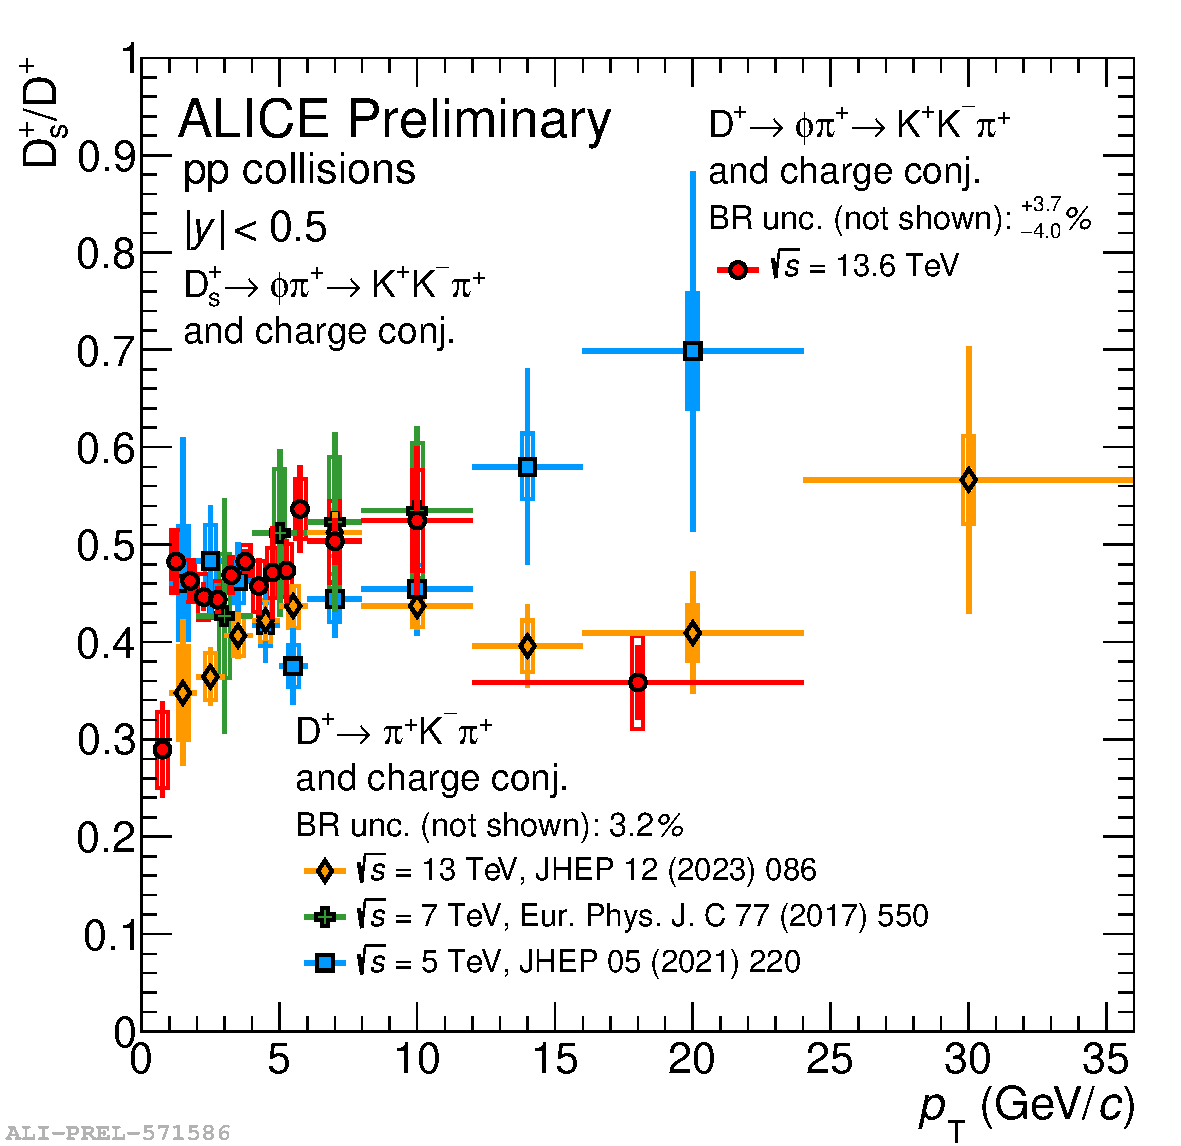
\includegraphics[width=0.7\textwidth]{Figures/Chapter 7/dsoverdpluscomparisonalice_0.pdf}
    \caption{\pt-differential \ds/\dpl production-yield ratio measured at midrapidity ($\lvert y\rvert<0.5$) in pp collisions by the ALICE Collaboration. The results obtained in this Thesis at \thirteen (red) are compared with previous measurements in pp collisions at $\sqrt{s} = 5$, 7, and 13~\tev (blue, green, and orange, respectively).}
    \label{fig:dsdplvsenergy}
\end{figure}

Therefore, an enhancement in the production of strange hadrons might be expected with the increase in the energy available in the collision. The dependence on the centre-of-mass energy of the \ds/\dpl production-yield ratio can be studied by comparing the results obtained in this Thesis in pp collisions at \thirteen with those obtained, in the same rapidity window of \mbox{$\lvert y\rvert<0.5$}, by the ALICE Collaboration in pp collisions at the centre-of-mass energies of $\sqrt{s} = 5$, 7, and 13~\tev (taken from Refs.~\cite{ALICE:2021mgk,ALICE:2017olh,ALICE:2023sgl}, respectively). Given the small difference of a few \tev between the considered measurements, a very small effect on the \ds/\dpl production-yield ratio is expected. Using the parametrisations of the charged-particle multiplicity density as a function of the centre-of-mass energy per nucleon pair of the collision reported in Ref~\cite{ALICE:2015juo} and shown in Fig.~\ref{fig:pseudorap_density}, a factor of about $(13.6/5.02)^{0.206} \sim 1.2$ is expected between the multiplicities measured at \thirteen and $\sqrt{s} = 5.02$~\tev (since the number of participating nucleons $N_\mathrm{part}$ in a pp collision is always 2: the two protons). 

The comparison is shown in Fig.~\ref{fig:dsdplvsenergy}, with red markers being used for the measurement performed in this Thesis. Thanks to the upgrade to the ALICE experimental apparatus~\cite{ALICE:2023udb}, a very large number of minimum-bias events was recorded. In one year of Run~3 data-taking, an integrated luminosity larger than that of the entire Run~2 was collected. In addition, previous measurements of the \ds/\dpl production-yield ratio reconstructed the \dpl meson through the $\dpl\rightarrow\pi^+\mathrm{K}^-\pi^+$ decay channel, which differs from that exploited in this analysis. Despite being characterised by a larger BR of \mbox{$(9.38\pm0.16)\times10^{-2}$}~\cite{pdg}, which leads to a larger amount of reconstructed \dpl mesons, the reconstruction through the same decay channel used for the \ds meson, $\dpl \rightarrow \mathrm{\phi\pi^+ \rightarrow K^+K^-\pi^+}$, allows for the cancellation of some of the systematic uncertainties in the \ds/\dpl ratio. Thereby, a high-precision measurement of the \ds/\dpl production-yield ratio was achieved in this Thesis. Both statistical and systematic uncertainties have been significantly reduced with respect to previous results. The \pt reach of the measurement has been extended to lower values, down to $\pt=0.5$~\gevc, and narrower \pt intervals have been analysed. At higher \pt, the worse \pt resolution on the tracks due to the increase of the electric field distortions in the TPC is more impactful, and the uncertainties increase. For the same reason, the \pt reach of the measurement is limited to $\pt<24$~\gevc, with no improvements in the granularity of the measurement at high \pt. The comparison with previous measurements at midrapidity performed by the ALICE Collaboration at the centre-of-mass energies of $\sqrt{s} = 5$, 7, and 13~\tev shows no significant dependence on the centre-of-mass energy, with results being compatible within uncertainties across the whole analysed \pt and \sqs ranges. The comparison with the results obtained at \mbox{$\sqs=13$~\tev} shows that a slightly larger \ds/\dpl production-yield ratio is measured at low \pt at \mbox{\thirteen}. However, the large uncertainties in the previous measurement prevent any firm conclusion on any energy dependence of the observable. In addition, large fluctuations may be present in the \ds and \dpl measurements at $\sqrt{s} = 13$~\tev, as can be deduced from the different trends of their production-yield ratio to the \dz meson compared to that measured at $\sqrt{s} = 5.02$~\tev. 

\section{Dependence on rapidity}
\begin{figure} 
    \centering
    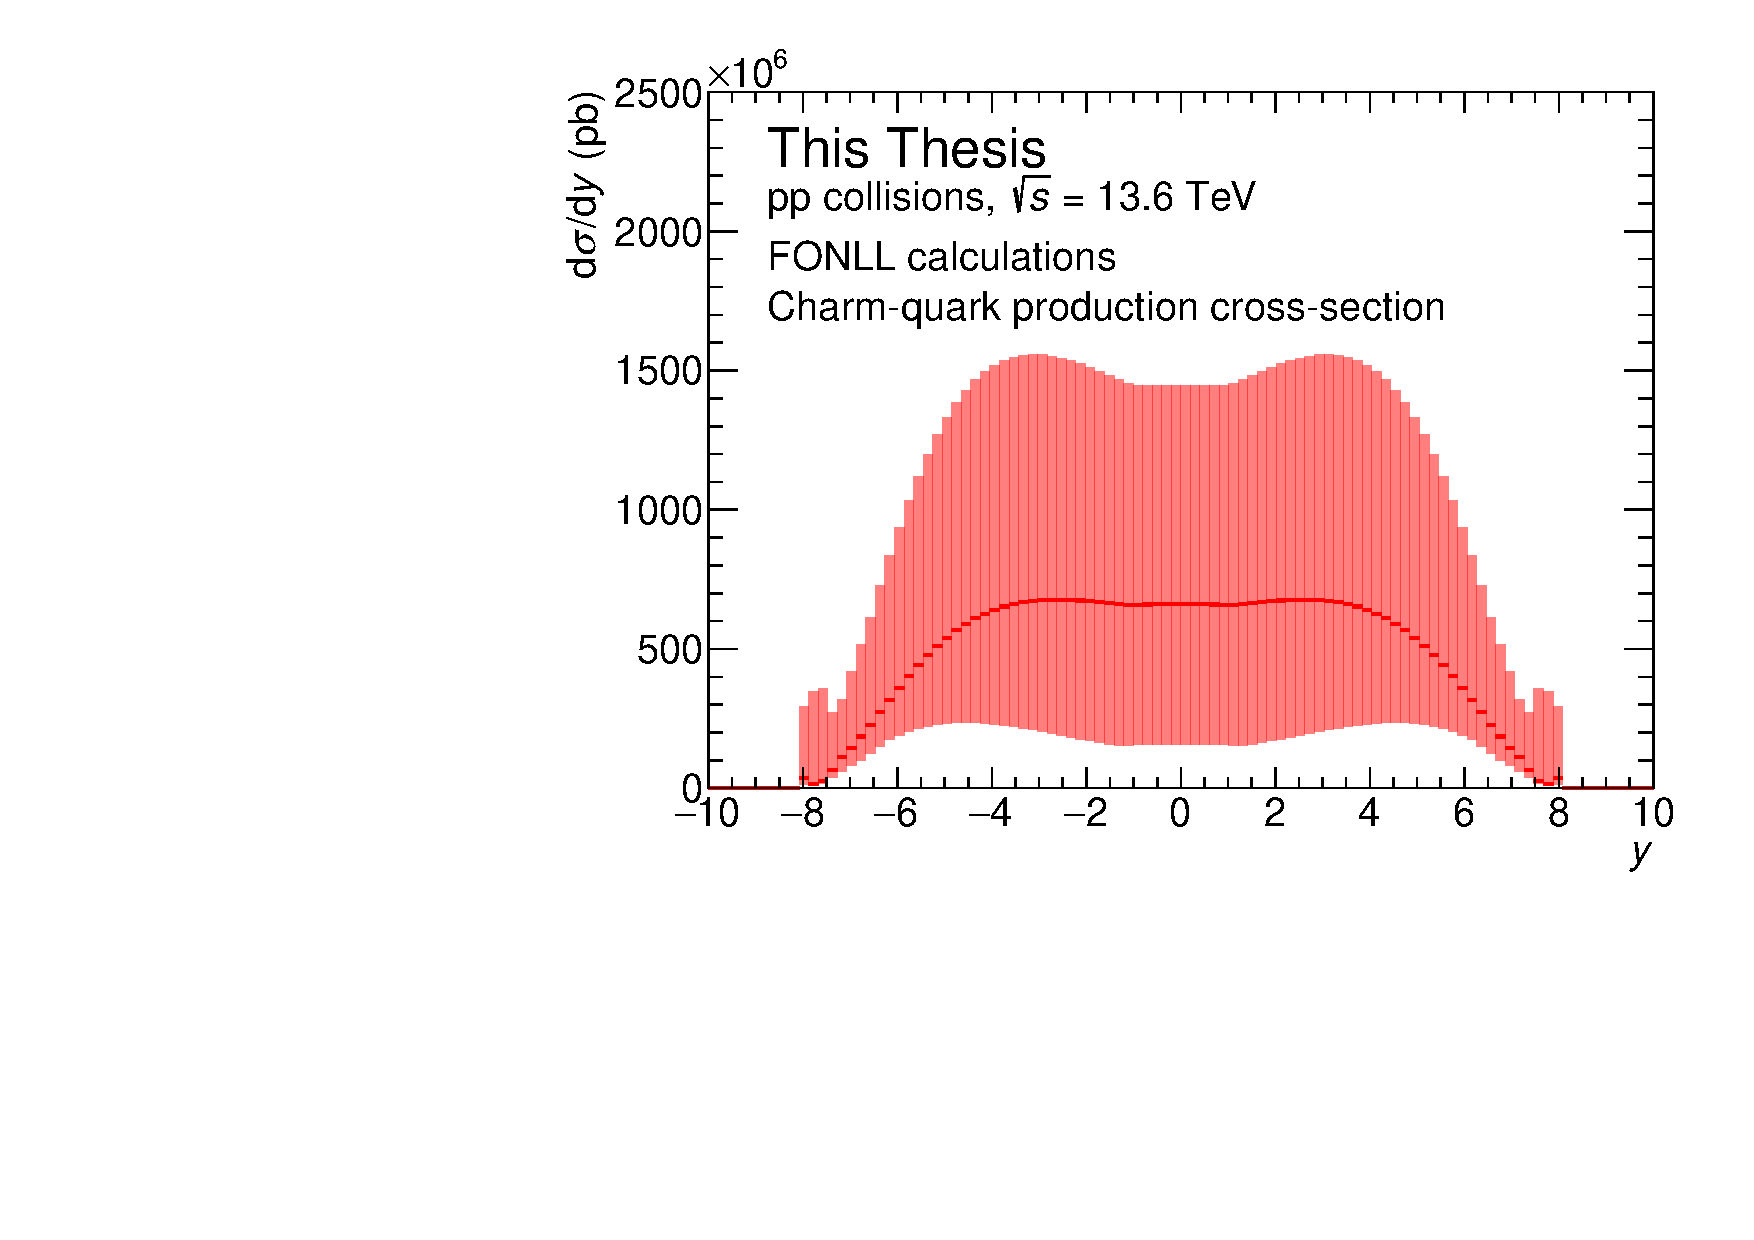
\includegraphics[width=0.7\textwidth]{Figures/Chapter 7/FONLLVsY.pdf}
    \caption{$y$-differential charm-quark production cross-section in  pp collisions at \thirteen predicted by FONLL~\cite{Cacciari:1998it} calcualations.}
    \label{fig:FONLLVsY}
\end{figure}
Measurements of the \ds/\dpl production-yield ratio in different rapidity intervals can provide further insights into the hadronisation mechanism. At forward rapidities, the production of particles closer to the beam remnants is probed. In this phase space region, interactions may occur between the fragments of the colliding hadrons and the partons produced in the hard-scattering processes. Therefore, the parton shower and the hadronisation might differ from those at midrapidity. Measurements performed at forward rapidity by colliding a beam of 340~~\gevc $\pi^-$ on a nuclear target at the SPS by the WA82 Collaboration~\cite{WA82:1993ghz} and by colliding a beam of $\pi^\pm$, $\mathrm{K^\pm}$, or protons on a nuclear target at the low energy of 250~\gev by the E769 Collaboration at Fermilab~\cite{E769:1996jqf} indicated the presence of an asymmetric production of leading and subleading charm particles. The term \emph{leading} particle refers in this context to a charm particle that shares at least one light quark or antiquark flavour with the beam particle. On the contrary, recent measurements performed by the ALICE Collaboration demonstrated a balance in the production of particles and antiparticles at midrapidity~\cite{ALICE:2023ulv}. This suggests that the hadronisation may undergo a change in the vicinity of the beam remnants. These asymmetries at rapidities close to the beam rapidity can be interpreted in the framework of hadronisation via coalescence, by assuming that the charm quark hadronises via recombination with some other quarks belonging to the beam remnants~\cite{Norrbin:1998bw,Norrbin:2000zc}. At LHC energies, rapidities of around 10 in the laboratory frame are reached by both colliding protons. FONLL calculations~\cite{Cacciari:1998it} for the $y$-differential charm-quark production cross-section in pp collisions at \thirteen predict an almost rapidity-independent cross-section for charm hadron production in $\lvert y\rvert<4$ and a steeply-falling trend with rapidity for $\lvert y\rvert>4$, as shown in Fig.~\ref{fig:FONLLVsY}. The LHCb experimental apparatus is able to perform measurements at forward rapidity in $2.0<y<4.5$, but does not reach the large $y$ values of the beam remnants. Therefore, it is not expected to observe significant differences between measurements performed in the ALICE and LHCb rapidity ranges. 

\begin{figure}[tb]
    \centering
    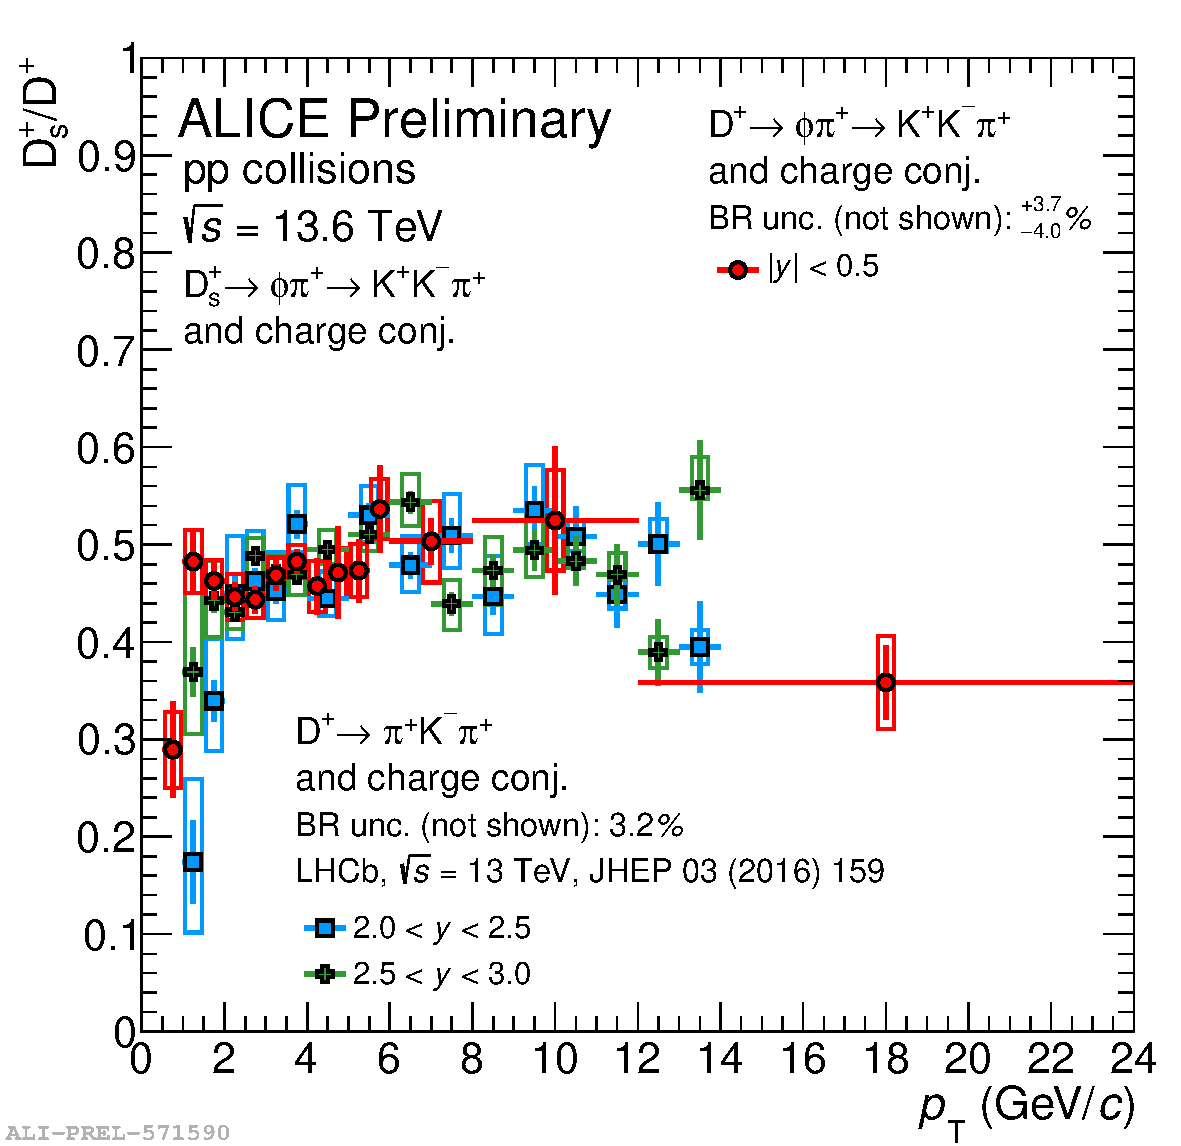
\includegraphics[width=0.48\textwidth]{Figures/Chapter 7/dsoverdpluscomparisonlhcb.pdf}
    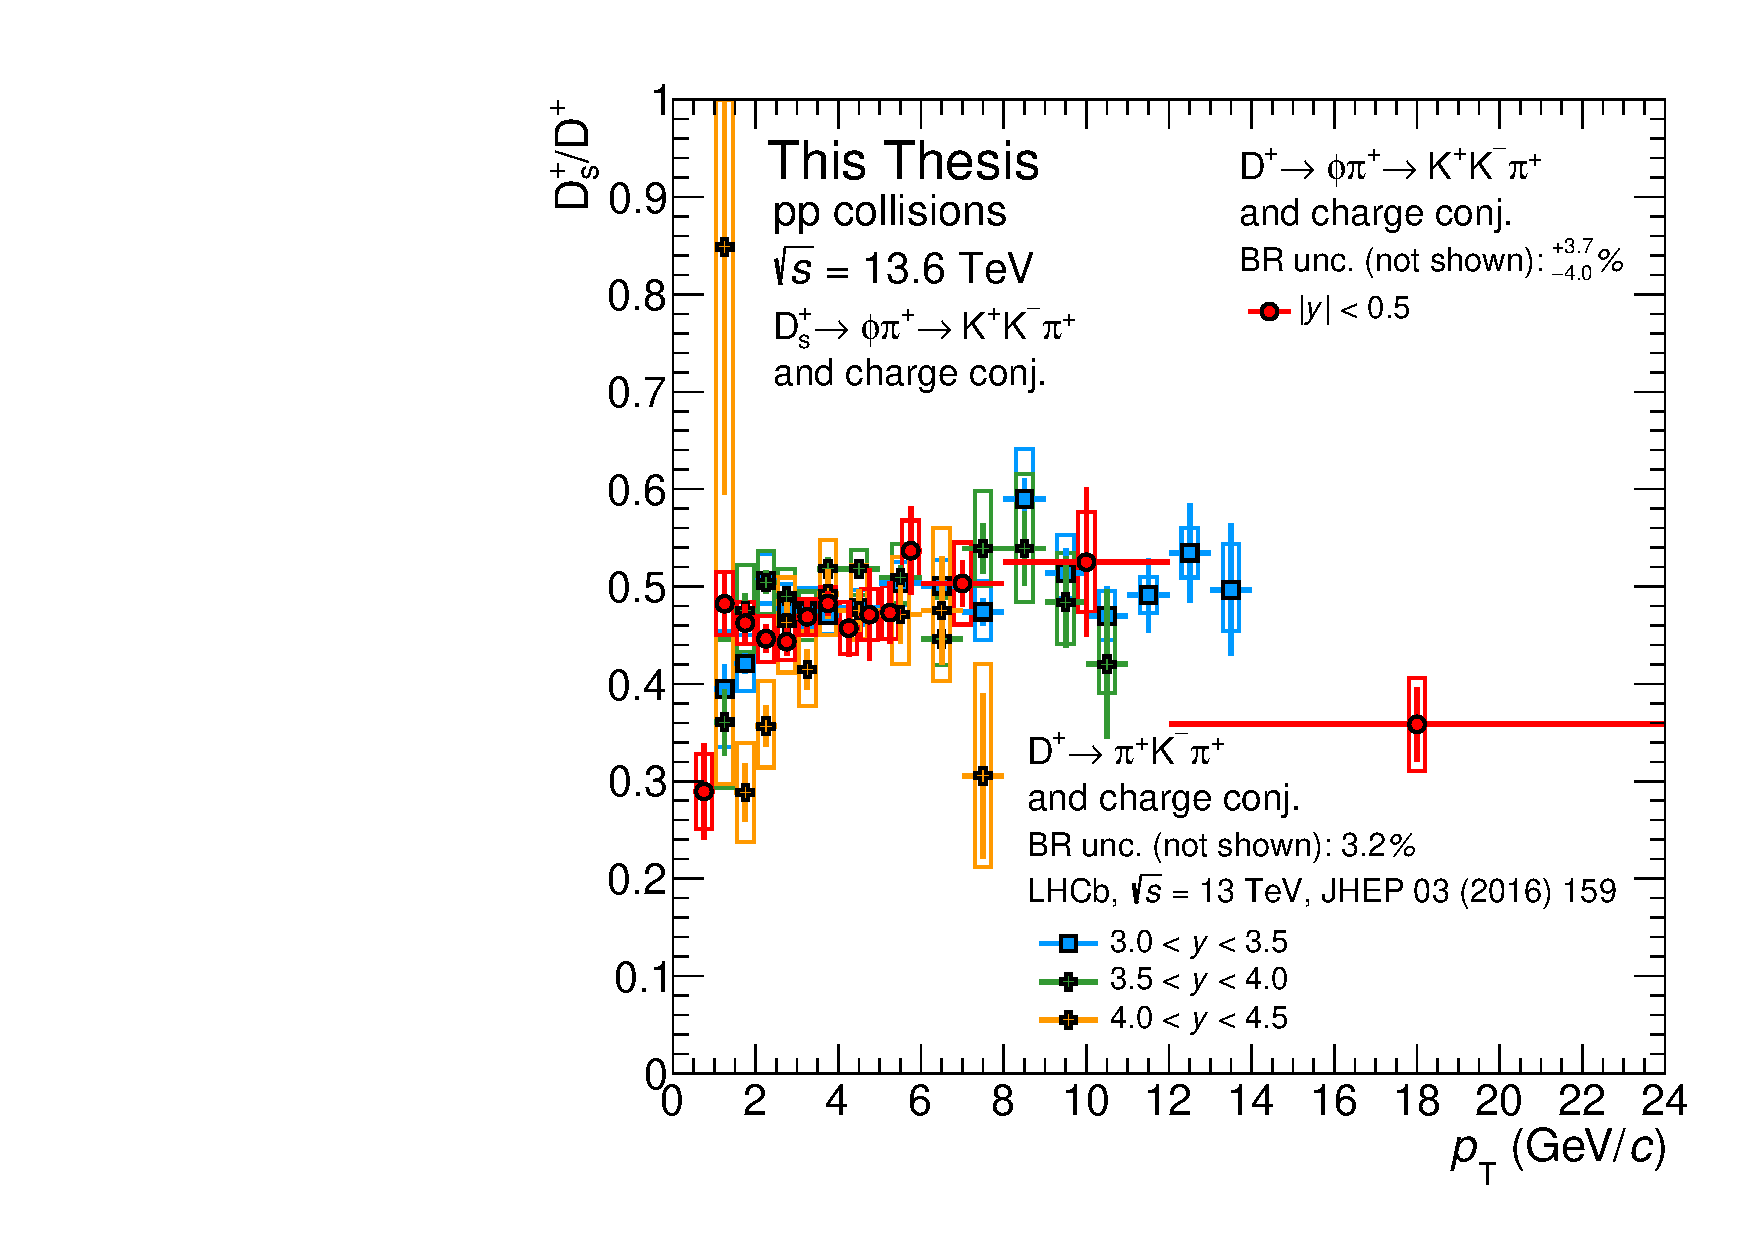
\includegraphics[width=0.48\textwidth]{Figures/Chapter 7/DsOverDplusComparisonLHCbHighRap.pdf}
    \caption{\pt-differential \ds/\dpl production-yield ratio measured at midrapidity ($\lvert y\rvert<0.5$) in pp collisions at \thirteen by the ALICE Collaboration (red), obtained in this Thesis, compared with previous measurement in pp collisions at $\sqs=13$~\tev performed by the LHCb Collaboration in the forward-rapidity intervals of $2.0<y<2.5$ (blue) and $2.5<y<3.0$ (green) in the left panel and the $3.0<y<3.5$ (blue), $3.5<y<4.0$ (green), and $4.0<y<4.5$ (orange) rapidity intervals in the right panel.}
    \label{fig:dsdplvsrapidity}
\end{figure}

The rapidity dependence of the \ds/\dpl produciton-yield ratio can be investigated by comparing the measurement at midrapidity ($\lvert y\rvert<0.5$) performed in this Thesis in pp collisions at \thirteen with those performed at forward rapidities by the LHCb Collaboration~\cite{LHCb:2015swx} at a similar centre-of-mass energy of $\sqs=13$~\tev. Given the energy-independence of the observable which has been discussed above, it is possible to directly compare the two measurements. Figure~\ref{fig:dsdplvsrapidity} shows the comparison between the \ds/\dpl production-yield ratio measured in this work compared to that from the LHCb Collaboration measured in pp collisions in the $2.0<y<2.5$ and $2.5<y<3.0$ rapidity intervals (left panel), and in the $3.0<y<3.5$, $3.5<y<4.0$, and $4.0<y<4.5$ rapidity intervals (right panel). Thanks to the large dataset available and the reconstruction of the two D-meson species through the same decay channel, the uncertainties of the measurement are significantly smaller than those of the results obtained by the LHCb Collaboration across a wide \pt range. In addition, the \pt reach of the measurement is extended to lower values. The results obtained at midrapidity and forward rapidity show a similar trend, with the \ds/\dpl production-yield ratios being compatible within uncertainties across the whole studied \pt and $y$ range. The comparison between the results obtained at midrapidity and forward rapidity shows no significant dependence of the \ds/\dpl production-yield ratio on the rapidity of the measurement.


Other measurements performed at forward rapidity by the LHCb Collaboration in p--Pb collisions at $\snn=8.16$~\tev~\cite{LHCb:2023rpm} present an enhancement of the \ds/\dpl production-yield ratio as a function of the charged-particle multiplicity across the studied \mbox{$2<\pt<12$~\gevc} interval. These results were obtained by determining the charged-particle multiplicity of the collision using a detector capable of measuring the number of produced particles in the same rapidity interval in which the D-meson production is measured. This may lead to possible biases in the measurement, as heavy-flavour hadrons are typically produced in jets, and auto-correlations between the charged-particle multiplicity and the D-meson production may be present. This could also cause the different slope of the measured \ds/\dpl production between forward and backward rapidities. The ALICE apparatus overcomes these limitations, as the charged-particle multiplicity of events containing D mesons in the central barrel can be measured with forward-rapidity detectors, such as the FV0 and the two arrays of the FT0 detector. Therefore, future measurements of the multiplicity dependence of the \ds/\dpl production-yield ratio in pp collisions performed by the ALICE Collaboration are expected to provide a more accurate determination of the observable, and to be less affected by biases due to the presence of auto-correlations between the D-meson production and the charged-particle multiplicity of the collision. 
\section{Comparison to models}
\begin{figure}[htb]
    \centering
    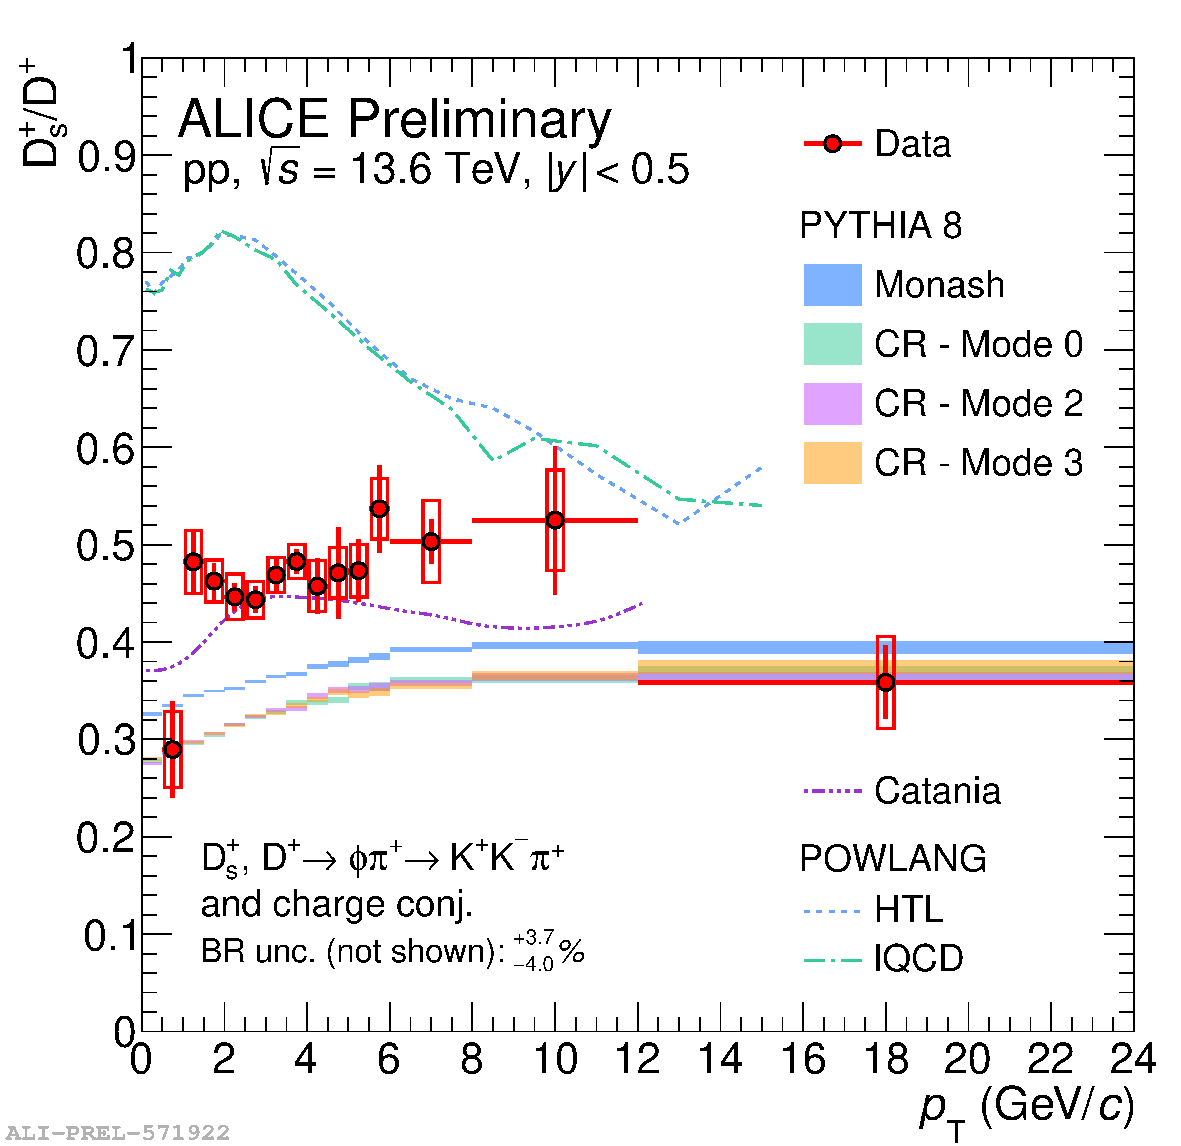
\includegraphics[width=0.7\textwidth]{Figures/Chapter 7/dsoverdpluscomparisonmodels_0.pdf}
    \caption{\pt-differential \ds/\dpl production-yield ratio measured at midrapidity ($\lvert y\rvert<0.5$) in pp collisions at \thirteen by the ALICE Collaboration. The results obtained in this Thesis (red) are compared with different theoretical predictions.}
    \label{fig:dsdplvsmodels}
\end{figure}
The \ds/\dpl production-yield ratio can be used to test the validity of models describing the production of the two D-meson species, and set constraints on their description of the hadronisation process. Figure~\ref{fig:dsdplvsmodels} presents a comparison between the \ds/\dpl production-yield ratio measured in this Thesis at midrapidity ($\lvert y\rvert<0.5$) in pp collisions at \thirteen with the ALICE experiment (red markers) and theoretical predictions. 

Predictions from \textsc{Pythia}~8~\cite{Bierlich:2022pfr} are reported using the Monash 2013 tune~\cite{Skands:2014pea} (blue filled boxes), which tunes its hadronisation description on results from \ee collisions, and CR tunes implementing colour-reconnections beyond the leading-colour approximation~\cite{Christiansen:2015yqa}. The width of the \textsc{Pythia}~8 bands in Fig.~\ref{fig:dsdplvsmodels} represents the statistical uncertainty due to the limited amount of simulated pp collision events. Three colour reconnection modes (Mode 0,2,3) are reported in green, violet, and orange, and present similar trends with \pt, with values compatible within uncertainties. \textsc{Pythia}~8 predictions with Monash 2013 tune present a similar dependence on \pt, with a predicted \ds/\dpl production-yield ratio that is larger than that with colour-reconnections beyond the leading-colour approximation. Nonetheless, the four predictions underestimate the measured \ds/\dpl ratio, by a factor of about 1.5 at intermediate \pt. This discrepancy is also observed in the measurement of the \pt integrated $\ds/\mathrm{D^0}$ and $\dpl/\mathrm{D^0}$ production-yield ratio in pp collisions at 5.02~\tev performed by the ALICE Collaboration~\cite{ALICE:2021dhb}, where the same \textsc{Pythia}~8 predictions were found to slightly underestimate the \ds-meson production and overestimate that of \dpl mesons.

Predictions from the Catania model~\cite{Minissale:2020bif}, which assumes the production of small droplets of QGP in pp collisions, implementing both the coalescence and fragmentation mechanisms for charm quark hadronisation, are reported with a violet dot-dashed line. The model provides a good description of the \ds/\dpl production-yield ratio, managing to reproduce both the magnitude and the general trend with transverse momentum in the range $2<\pt<6$~\gevc, showing some tension with the data at low and high \pt. 

Lastly, predictions from POWLANG~\cite{Beraudo:2023nlq}, are also reported. Similarly to the Catania model, POWLANG assumes the formation of a small deconfined system in pp collisions, and the same in-medium hadronization mechanism developed for heavy-ion collisions, based on local colour neutralisation via the formation of clusters of quarks and diquarks, is employed. Two sets of predictions are reported, employing transport coefficients calculated with weak-coupling calculations~\cite{Braaten:1989mz} (Hard-Thermal-Loop, HTL) and lattice-QCD simulations~\cite{Altenkort:2023oms}, using blue and green dashed lines, respectively. Both predictions overestimate the measured \ds/\dpl production-yield ratio, by a factor of about 1.5 at intermediate \pt. In addition, a strong decreasing trend with \pt is predicted in the $2<\pt<12$~\gevc, but not observed in the data. These discrepancies are also observed in the measurement of the \pt-differential $\ds/\mathrm{D^0}$ production-yield ratio in pp collisions at 5.02~\tev performed by the ALICE Collaboration~\cite{Beraudo:2023nlq}, where the POWLANG predictions overestimate the \ds-meson production, with similar differences in the description of the \pt-dependence, while an accurate description of the \dpl/\dz production-yield ratio is achieved.








%\begin{table}
%    \centering
%    \begin{tabular}{c|cccccc}
%        \toprule
%        Mesone & Massa (\mevcc) & $c\tau (\SI{}{\micro\meter})$ & Canale di %decadimento & BR \\
%        \midrule
%        $\mathrm{D}^0$ & $1864.84 \pm 0.05$ & $123 \pm 3$ & $\mathrm{K}^-\pi^+$ & $%(3.947 \pm 0.030)\%$ \\ 
%        $\mathrm{D}^+$ & $1869.66 \pm 0.05$ & $310 \pm 2$ & $\pi^+\mathrm{K}^-\pi^%+$ & $(9.38 \pm 0.16)\%$ \\
%        & & & $\phi\pi^+\rightarrow \mathrm{K}^+\mathrm{K}^-\pi^+$ & $(2.69^{+0.07}_%{-0.08})\times10^{-3}$ \\
%        $\mathrm{D^+_s}$ & $1968.35 \pm 0.07$ & $150 \pm 6$ & $\phi\pi^+\rightarrow %\mathrm{K}^+\mathrm{K}^-\pi^+$ & $(2.21 \pm 0.06)\%$ \\
%        \midrule
%        $\mathrm{B^0}$ & $5279.72 \pm 0.08$ & $455 \pm 12$ & $\mathrm{D}^-\pi^+$ & $%(2.51 \pm 0.08)\times10^{-3}$ \\
%        & & & $\mathrm{D}^-\mathrm{K}^+$ & $(2.05 \pm 0.08)\times10^{-4}$ \\
%        $\mathrm{B^+}$ & $5279.41 \pm 0.07$ & $491 \pm 12$ & $\mathrm{\overline{D}}%^0\pi^+$ & $(4.61 \pm 0.10)\times10^{-3}$ \\
%        & & & $\mathrm{\overline{D}}^0\mathrm{K}^+$ & $(3.64 \pm 0.15)\times10^{-4}$ %\\
%        $\mathrm{B^0_s}$ & $5366.93 \pm 0.10$ & $456 \pm 15$ & $\mathrm{D_s^-}\pi^%+$ & $(2.98 \pm 0.14)\times10^{-3}$ \\
%        & & & $\mathrm{D_s^\mp}\mathrm{K}^\pm$ & $(2.25 \pm 0.12)\times10^{-4}$ \\
%        \bottomrule
%    \end{tabular}
%\end{table}